\begin{table}[p]
\begin{footnotesize}
    \begin{tabular}{c|cc|ccc|ccc}
     \hline
                       & SCM  & Tyler & HSD-CM & MhD-CM & PD-CM & HSD-wCM & MhD-wCM & PD-wCM \\ \hline
    Bivariate $t_5$    & 1.46 & 1.50  & 1.97   & 1.54   & 1.99  & 2.09    & 1.57    & 2.11   \\
    Bivariate $t_6$    & 0.97 & 1.00  & 1.37   & 1.12   & 1.40  & 1.45    & 1.19    & 1.49   \\
    Bivariate $t_{10}$ & 0.65 & 0.67  & 0.96   & 0.88   & 1.02  & 1.02    & 0.94    & 1.10   \\
    Bivariate $t_{15}$ & 0.57 & 0.59  & 0.87   & 0.82   & 0.94  & 0.92    & 0.87    & 1.00   \\
    Bivariate $t_{25}$ & 0.54 & 0.55  & 0.79   & 0.75   & 0.88  & 0.85    & 0.81    & 0.95   \\
    BVN   & 0.49 & 0.50  & 0.73   & 0.71   & 0.82  & 0.77    & 0.75    & 0.88   \\ \hline
    \end{tabular}
\end{footnotesize}
\caption{Asymptotic efficiencies relative to sample covariance matrix for $p=2$}
\label{table:AREtable}
\end{table}

\begin{table}[p]
\begin{footnotesize}
    \begin{tabular}{c|cc|ccc|ccc}
    \hline
    $F$ = Bivariate $t_5$    & SCM  & Tyler & HSD-CM & MhD-CM & PD-CM & HSD-wCM & MhD-wCM & PD-wCM \\ \hline
    $n$=20                   & 0.80 & 0.83  & 0.95   & 0.95   & 0.89  & 1.00    & 0.96    & 0.89   \\
    $n$=50                   & 0.86 & 0.90  & 1.25   & 1.10   & 1.21  & 1.32    & 1.13    & 1.25   \\
    $n$=100                  & 1.02 & 1.04  & 1.58   & 1.20   & 1.54  & 1.67    & 1.24    & 1.63   \\
    $n$=300                  & 1.24 & 1.28  & 1.81   & 1.36   & 1.82  & 1.93    & 1.44    & 1.95   \\
    $n$=500                  & 1.25 & 1.29  & 1.80   & 1.33   & 1.84  & 1.91    & 1.39    & 1.97   \\ \hline
    $F$ = Bivariate $t_6$    & SCM  & Tyler & HSD-CM & MhD-CM & PD-CM & HSD-wCM & MhD-wCM & PD-wCM \\ \hline
    $n$=20                   & 0.77 & 0.79  & 0.92   & 0.92   & 0.86  & 0.96    & 0.92    & 0.85   \\
    $n$=50                   & 0.76 & 0.78  & 1.11   & 1.00   & 1.08  & 1.17    & 1.03    & 1.13   \\
    $n$=100                  & 0.78 & 0.79  & 1.27   & 1.06   & 1.33  & 1.35    & 1.11    & 1.41   \\
    $n$=300                  & 0.88 & 0.91  & 1.29   & 1.09   & 1.35  & 1.38    & 1.15    & 1.45   \\
    $n$=500                  & 0.93 & 0.96  & 1.37   & 1.13   & 1.40  & 1.44    & 1.19    & 1.48   \\ \hline
    $F$ = Bivariate $t_{10}$ & SCM  & Tyler & HSD-CM & MhD-CM & PD-CM & HSD-wCM & MhD-wCM & PD-wCM \\ \hline
    $n$=20                   & 0.70 & 0.72  & 0.83   & 0.84   & 0.77  & 0.89    & 0.87    & 0.79   \\
    $n$=50                   & 0.58 & 0.60  & 0.90   & 0.84   & 0.86  & 0.95    & 0.88    & 0.91   \\
    $n$=100                  & 0.57 & 0.59  & 0.92   & 0.87   & 0.97  & 0.98    & 0.90    & 1.03   \\
    $n$=300                  & 0.62 & 0.64  & 0.93   & 0.85   & 0.99  & 0.99    & 0.91    & 1.06   \\
    $n$=500                  & 0.62 & 0.65  & 0.93   & 0.86   & 1.00  & 1.00    & 0.92    & 1.08   \\ \hline
    $F$ = Bivariate $t_{15}$ & SCM  & Tyler & HSD-CM & MhD-CM & PD-CM & HSD-wCM & MhD-wCM & PD-wCM \\ \hline
    $n$=20                   & 0.63 & 0.66  & 0.76   & 0.78   & 0.72  & 0.81    & 0.81    & 0.73   \\
    $n$=50                   & 0.52 & 0.52  & 0.79   & 0.75   & 0.80  & 0.84    & 0.79    & 0.85   \\
    $n$=100                  & 0.51 & 0.52  & 0.83   & 0.77   & 0.88  & 0.88    & 0.81    & 0.94   \\
    $n$=300                  & 0.55 & 0.56  & 0.84   & 0.79   & 0.91  & 0.89    & 0.84    & 0.98   \\
    $n$=500                  & 0.56 & 0.59  & 0.85   & 0.80   & 0.93  & 0.91    & 0.86    & 0.99   \\ \hline
    $F$ = Bivariate $t_{25}$ & SCM  & Tyler & HSD-CM & MhD-CM & PD-CM & HSD-wCM & MhD-wCM & PD-wCM \\ \hline
    $n$=20                   & 0.63 & 0.65  & 0.77   & 0.79   & 0.74  & 0.80    & 0.81    & 0.74   \\
    $n$=50                   & 0.49 & 0.50  & 0.73   & 0.71   & 0.76  & 0.78    & 0.75    & 0.80   \\
    $n$=100                  & 0.45 & 0.46  & 0.73   & 0.69   & 0.81  & 0.78    & 0.73    & 0.87   \\
    $n$=300                  & 0.51 & 0.52  & 0.78   & 0.75   & 0.87  & 0.83    & 0.79    & 0.94   \\
    $n$=500                  & 0.53 & 0.55  & 0.79   & 0.75   & 0.87  & 0.84    & 0.80    & 0.94   \\ \hline
    $F$ = BVN                & SCM  & Tyler & HSD-CM & MhD-CM & PD-CM & HSD-wCM & MhD-wCM & PD-wCM \\ \hline
    $n$=20                   & 0.56 & 0.60  & 0.69   & 0.71   & 0.67  & 0.73    & 0.74    & 0.68   \\
    $n$=50                   & 0.42 & 0.43  & 0.66   & 0.66   & 0.70  & 0.71    & 0.69    & 0.75   \\
    $n$=100                  & 0.42 & 0.43  & 0.69   & 0.66   & 0.77  & 0.74    & 0.71    & 0.83   \\
    $n$=300                  & 0.47 & 0.49  & 0.71   & 0.69   & 0.82  & 0.76    & 0.73    & 0.88   \\
    $n$=500                  & 0.48 & 0.50  & 0.73   & 0.71   & 0.83  & 0.78    & 0.76    & 0.89   \\ \hline
    \end{tabular}
\end{footnotesize}
\caption{Finite sample efficiencies of several scatter matrices: $p=2$}
\label{table:FSEtable2}
\end{table}

\begin{table}[p]
\begin{footnotesize}
   \begin{tabular}{c|cc|ccc|ccc}
    \hline
    3-variate $t_5$    & SCM  & Tyler & HSD-CM & MhD-CM & PD-CM & HSD-wCM & MhD-wCM & PD-wCM \\ \hline
    $n$=20             & 0.96 & 0.97  & 1.06   & 1.03   & 0.99  & 1.07    & 1.06    & 0.97   \\
    $n$=50             & 1.07 & 1.08  & 1.28   & 1.20   & 1.18  & 1.33    & 1.23    & 1.20   \\
    $n$=100            & 1.12 & 1.15  & 1.49   & 1.31   & 1.40  & 1.57    & 1.38    & 1.48   \\
    $n$=300            & 1.49 & 1.54  & 2.09   & 1.82   & 2.07  & 2.19    & 1.93    & 2.18   \\
    $n$=500            & 1.60 & 1.66  & 2.18   & 1.87   & 2.21  & 2.27    & 1.95    & 2.30   \\ \hline
    3-variate $t_6$    & SCM  & Tyler & HSD-CM & MhD-CM & PD-CM & HSD-wCM & MhD-wCM & PD-wCM \\ \hline
    $n$=20             & 0.90 & 0.92  & 1.00   & 0.99   & 0.95  & 1.02    & 1.01    & 0.94   \\
    $n$=50             & 0.95 & 0.96  & 1.16   & 1.09   & 1.09  & 1.21    & 1.14    & 1.11   \\
    $n$=100            & 0.98 & 0.99  & 1.32   & 1.22   & 1.25  & 1.38    & 1.27    & 1.29   \\
    $n$=300            & 1.10 & 1.14  & 1.57   & 1.40   & 1.58  & 1.62    & 1.47    & 1.64   \\
    $n$=500            & 1.17 & 1.20  & 1.57   & 1.43   & 1.60  & 1.63    & 1.51    & 1.67   \\ \hline
    3-variate $t_{10}$ & SCM  & Tyler & HSD-CM & MhD-CM & PD-CM & HSD-wCM & MhD-wCM & PD-wCM \\ \hline
    $n$=20             & 0.87 & 0.88  & 0.95   & 0.94   & 0.90  & 0.97    & 0.98    & 0.89   \\
    $n$=50             & 0.77 & 0.79  & 0.96   & 0.92   & 0.94  & 0.99    & 0.96    & 0.95   \\
    $n$=100            & 0.75 & 0.76  & 1.02   & 0.95   & 1.01  & 1.06    & 1.00    & 1.05   \\
    $n$=300            & 0.73 & 0.75  & 1.03   & 0.98   & 1.10  & 1.08    & 1.03    & 1.15   \\
    $n$=500            & 0.73 & 0.76  & 1.02   & 0.98   & 1.09  & 1.06    & 1.02    & 1.14   \\ \hline
    3-variate $t_{15}$ & SCM  & Tyler & HSD-CM & MhD-CM & PD-CM & HSD-wCM & MhD-wCM & PD-wCM \\ \hline
    $n$=20             & 0.84 & 0.86  & 0.92   & 0.92   & 0.89  & 0.94    & 0.94    & 0.87   \\
    $n$=50             & 0.75 & 0.76  & 0.92   & 0.90   & 0.90  & 0.96    & 0.94    & 0.93   \\
    $n$=100            & 0.66 & 0.67  & 0.91   & 0.87   & 0.95  & 0.96    & 0.92    & 1.00   \\
    $n$=300            & 0.61 & 0.64  & 0.90   & 0.87   & 1.00  & 0.93    & 0.91    & 1.04   \\
    $n$=500            & 0.65 & 0.67  & 0.89   & 0.87   & 0.99  & 0.93    & 0.91    & 1.03   \\ \hline
    3-variate $t_{25}$ & SCM  & Tyler & HSD-CM & MhD-CM & PD-CM & HSD-wCM & MhD-wCM & PD-wCM \\ \hline
    $n$=20             & 0.78 & 0.79  & 0.87   & 0.89   & 0.87  & 0.89    & 0.92    & 0.86   \\
    $n$=50             & 0.70 & 0.71  & 0.88   & 0.86   & 0.88  & 0.91    & 0.90    & 0.90   \\
    $n$=100            & 0.61 & 0.63  & 0.86   & 0.83   & 0.89  & 0.90    & 0.88    & 0.94   \\
    $n$=300            & 0.58 & 0.59  & 0.83   & 0.80   & 0.92  & 0.87    & 0.85    & 0.98   \\
    $n$=500            & 0.62 & 0.64  & 0.83   & 0.82   & 0.94  & 0.88    & 0.87    & 0.99   \\ \hline
    3-variate Normal   & SCM  & Tyler & HSD-CM & MhD-CM & PD-CM & HSD-wCM & MhD-wCM & PD-wCM \\ \hline
    $n$=20             & 0.76 & 0.78  & 0.85   & 0.87   & 0.84  & 0.87    & 0.90    & 0.83   \\
    $n$=50             & 0.66 & 0.67  & 0.82   & 0.81   & 0.84  & 0.86    & 0.86    & 0.86   \\
    $n$=100            & 0.56 & 0.58  & 0.77   & 0.75   & 0.83  & 0.82    & 0.79    & 0.87   \\
    $n$=300            & 0.53 & 0.55  & 0.75   & 0.74   & 0.85  & 0.79    & 0.78    & 0.90   \\
    $n$=500            & 0.56 & 0.58  & 0.76   & 0.76   & 0.87  & 0.80    & 0.80    & 0.92   \\ \hline
    \end{tabular}
\end{footnotesize}
\caption{Finite sample efficiencies of several scatter matrices: $p=3$}
\label{table:FSEtable3}
\end{table}

\begin{table}[p]
\begin{footnotesize}
    \begin{tabular}{c|cc|ccc|ccc}
    \hline
    4-variate $t_5$    & SCM  & Tyler & HSD-CM & MhD-CM & PD-CM & HSD-wCM & MhD-wCM & PD-wCM \\ \hline
    $n$=20             & 1.04 & 1.02  & 1.10   & 1.07   & 1.02  & 1.09    & 1.07    & 0.98   \\
    $n$=50             & 1.08 & 1.08  & 1.16   & 1.16   & 1.13  & 1.19    & 1.19    & 1.13   \\
    $n$=100            & 1.31 & 1.31  & 1.42   & 1.38   & 1.36  & 1.46    & 1.44    & 1.36   \\
    $n$=300            & 1.46 & 1.54  & 1.81   & 1.76   & 1.95  & 1.88    & 1.88    & 1.95   \\
    $n$=500            & 1.92 & 1.93  & 2.23   & 2.03   & 2.31  & 2.35    & 2.19    & 2.39   \\ \hline
    4-variate $t_6$    & SCM  & Tyler & HSD-CM & MhD-CM & PD-CM & HSD-wCM & MhD-wCM & PD-wCM \\ \hline
    $n$=20             & 1.00 & 1.05  & 1.03   & 1.05   & 1.00  & 1.04    & 1.04    & 0.95   \\
    $n$=50             & 1.03 & 1.01  & 1.13   & 1.12   & 1.11  & 1.19    & 1.17    & 1.10   \\
    $n$=100            & 1.08 & 1.12  & 1.25   & 1.23   & 1.27  & 1.24    & 1.25    & 1.22   \\
    $n$=300            & 1.34 & 1.36  & 1.64   & 1.52   & 1.60  & 1.67    & 1.61    & 1.68   \\
    $n$=500            & 1.26 & 1.34  & 1.55   & 1.49   & 1.60  & 1.65    & 1.61    & 1.69   \\ \hline
    4-variate $t_{10}$ & SCM  & Tyler & HSD-CM & MhD-CM & PD-CM & HSD-wCM & MhD-wCM & PD-wCM \\ \hline
    $n$=20             & 0.90 & 0.89  & 0.95   & 0.98   & 0.98  & 0.96    & 1.01    & 0.95   \\
    $n$=50             & 0.90 & 0.91  & 1.01   & 0.98   & 0.98  & 1.03    & 1.04    & 0.99   \\
    $n$=100            & 0.87 & 0.87  & 0.93   & 0.95   & 1.01  & 0.99    & 1.01    & 1.05   \\
    $n$=300            & 0.87 & 0.87  & 1.09   & 1.09   & 1.17  & 1.14    & 1.16    & 1.23   \\
    $n$=500            & 0.88 & 0.92  & 1.10   & 1.10   & 1.23  & 1.19    & 1.22    & 1.29   \\ \hline
    4-variate $t_{15}$ & SCM  & Tyler & HSD-CM & MhD-CM & PD-CM & HSD-wCM & MhD-wCM & PD-wCM \\ \hline
    $n$=20             & 0.92 & 0.90  & 0.94   & 0.94   & 0.96  & 0.95    & 0.97    & 0.89   \\
    $n$=50             & 0.82 & 0.83  & 0.88   & 0.91   & 0.93  & 0.88    & 0.93    & 0.93   \\
    $n$=100            & 0.84 & 0.87  & 0.92   & 0.95   & 1.00  & 0.93    & 0.96    & 1.00   \\
    $n$=300            & 0.73 & 0.75  & 0.96   & 0.99   & 1.10  & 1.00    & 1.06    & 1.12   \\
    $n$=500            & 0.73 & 0.76  & 0.95   & 0.96   & 1.06  & 0.94    & 0.97    & 1.06   \\ \hline
    4-variate $t_{25}$ & SCM  & Tyler & HSD-CM & MhD-CM & PD-CM & HSD-wCM & MhD-wCM & PD-wCM \\ \hline
    $n$=20             & 0.89 & 0.92  & 0.92   & 0.92   & 0.90  & 0.96    & 0.95    & 0.89   \\
    $n$=50             & 0.82 & 0.84  & 0.89   & 0.90   & 0.91  & 0.93    & 0.96    & 0.92   \\
    $n$=100            & 0.77 & 0.76  & 0.90   & 0.90   & 0.96  & 0.94    & 0.98    & 1.04   \\
    $n$=300            & 0.73 & 0.77  & 0.93   & 0.91   & 0.98  & 1.00    & 0.98    & 1.03   \\
    $n$=500            & 0.67 & 0.71  & 0.83   & 0.83   & 0.96  & 0.88    & 0.90    & 1.00   \\ \hline
    4-variate Normal   & SCM  & Tyler & HSD-CM & MhD-CM & PD-CM & HSD-wCM & MhD-wCM & PD-wCM \\ \hline
    $n$=20             & 0.82 & 0.84  & 0.87   & 0.90   & 0.91  & 0.89    & 0.93    & 0.89   \\
    $n$=50             & 0.80 & 0.81  & 0.87   & 0.88   & 0.88  & 0.88    & 0.92    & 0.88   \\
    $n$=100            & 0.68 & 0.71  & 0.80   & 0.85   & 0.91  & 0.82    & 0.86    & 0.92   \\
    $n$=300            & 0.61 & 0.63  & 0.82   & 0.85   & 0.93  & 0.86    & 0.91    & 0.96   \\
    $n$=500            & 0.60 & 0.64  & 0.77   & 0.80   & 0.90  & 0.82    & 0.86    & 0.96   \\ \hline
    \end{tabular}
\end{footnotesize}
\caption{Finite sample efficiencies of several scatter matrices: $p=4$}
\label{table:FSEtable4}
\end{table}

\begin{table}[p]
\centering
    \begin{tabular}{c|ccccc}
    \hline
    \begin{large} $q$ \end{large} & \multicolumn{5}{c}{Method of PCA}         \\ \cline{2-6}
    ~                   & CPCA     & SPCA & ROBPCA & MPCA & DPCA \\\hline 
    1                   & 0.188         & 0.549     & 0.410  & 0.514     & 0.662     \\
    2                   & 0.084         & 0.272     & 0.214  & 0.337     & 0.359     \\
    3                   & 0.044         & 0.182     & 0.121  & 0.227     & 0.237     \\
    4                   & 0.026         & 0.135     & 0.083  & 0.154     & 0.173     \\
    5                   & 0.018         & 0.099     & 0.054  & 0.098     & 0.115     \\
    6                   & 0.012         & 0.069     & 0.036  & 0.070     & 0.084     \\ \hline
    \end{tabular}
    \caption{Unexplained proportions of variability by PCA models with $q$ components for bus data}
    \label{table:bus_table1}
\end{table}

\begin{table}[p]
\centering
    \begin{tabular}{c|ccccc}
    \hline
    Quantile & \multicolumn{5}{c}{Method of PCA}         \\ \cline{2-6}
    ~                   & CPCA     & SPCA & ROBPCA & MPCA & DPCA \\\hline 
    10\%      & 1.9       & 1.2       & 1.2    & 1.0       & 1.2       \\
    20\%      & 2.3       & 1.6       & 1.6    & 1.3       & 1.6       \\
    30\%      & 2.8       & 1.8       & 1.8    & 1.7       & 1.9       \\
    40\%      & 3.2       & 2.2       & 2.1    & 2.1       & 2.3       \\
    50\%      & 3.7       & 2.6       & 2.5    & 3.1       & 2.6       \\
    60\%      & 4.4       & 3.1       & 3.0    & 5.9       & 3.2       \\
    70\%      & 5.4       & 3.8       & 3.9    & 25.1      & 3.9       \\
    80\%      & 6.5       & 5.2       & 4.8    & 86.1      & 4.8       \\
    90\%      & 8.2       & 9.0       & 10.9   & 298.2     & 6.9      \\
    Max       & 24        & 1037      & 1055   & 1037      & 980      \\\hline
    \end{tabular}
    \caption{Quantiles to squared distance from 3-principal component hyperplanes for bus data}
    \label{table:bus_table2}
\end{table}

\begin{figure}[p]
	\captionsetup{singlelinecheck=off}
	\centering
		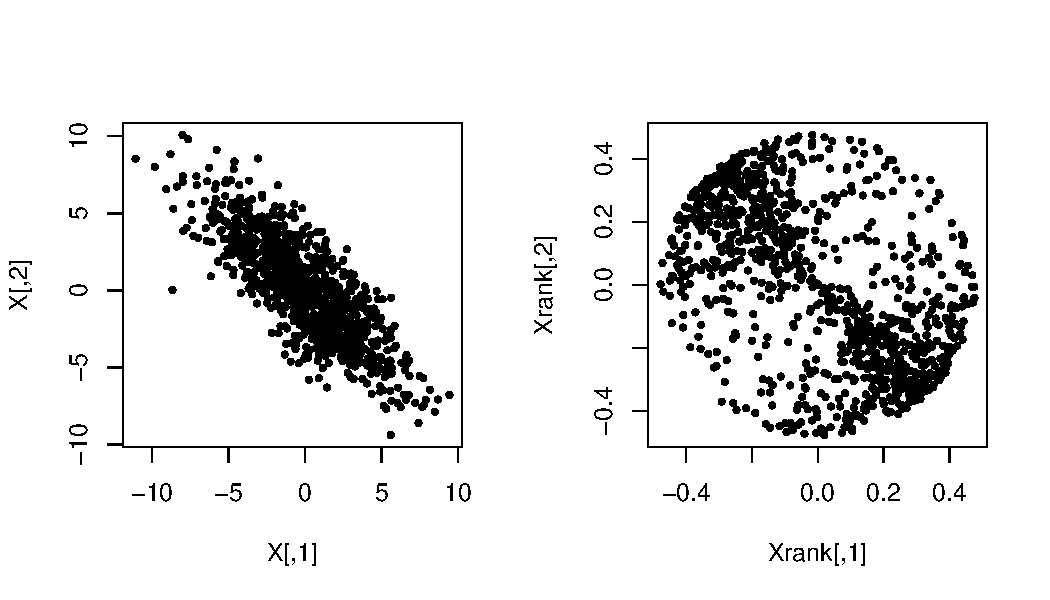
\includegraphics[height=6cm]{ranks.pdf}
	\caption{(Left) 1000 points randomly drawn from $\mathcal N_2\left((0,0)^T, \left(\protect\begin{smallmatrix} 5 & -4 \\ -4 & 5 \protect\end{smallmatrix}\right)\right) $ and (Right) their multivariate ranks based on halfspace depth}
	\label{fig:rankplot}
\end{figure}

\begin{figure}[p]
	\centering
		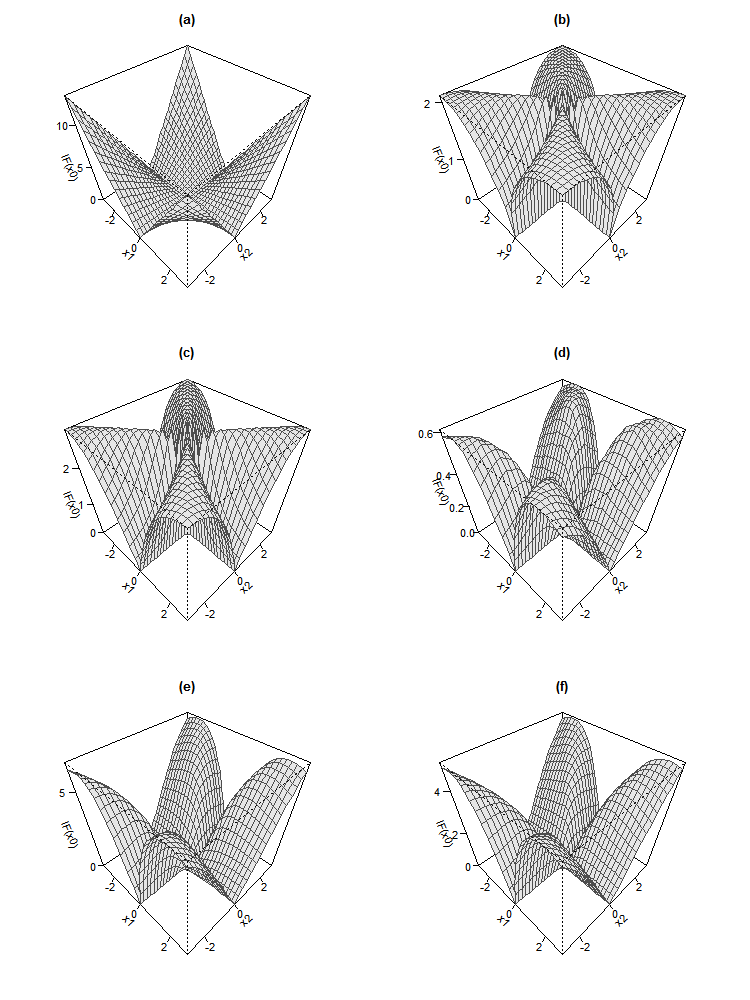
\includegraphics[width=12cm]{IFnorm.png}
	\caption{Plot of the norm of influence function for first eigenvector of (a) sample covariance matrix, (b) SCM, (c) Tyler's scatter matrix and DCMs for (d) Halfspace depth, (e) Mahalanobis depth, (f) Projection depth for a bivariate normal distribution with $\bfmu = {\bf 0}, \Sigma = \diag(2,1)$}
	\label{fig:IFnorm}
\end{figure}

\begin{figure}[t]
	\centering
		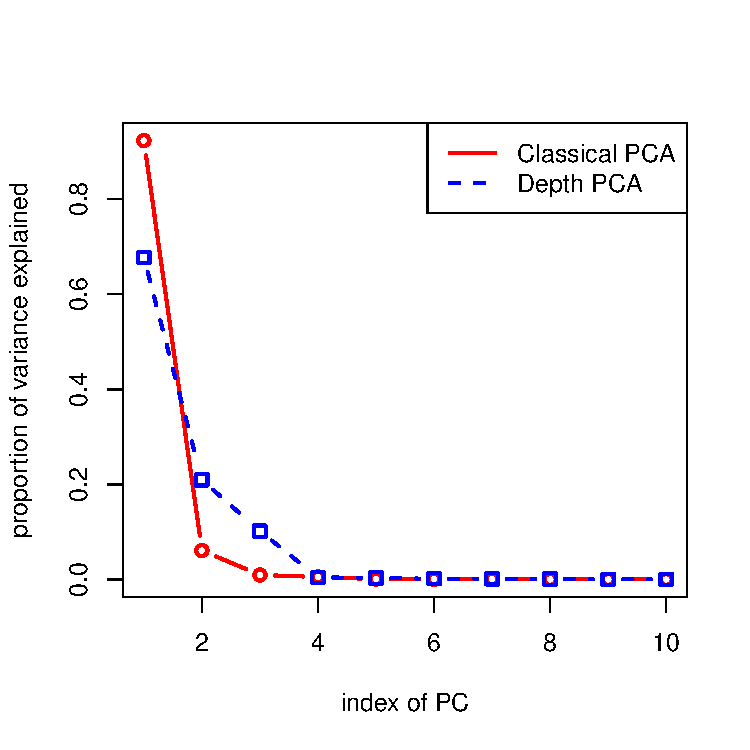
\includegraphics[height=6cm]{octane_screeplot.pdf}
	\caption{Explained variance proportions for two types of PCA on octane data}
	\label{fig:screeplot}
\end{figure}
\begin{figure}[h]
	\centering
		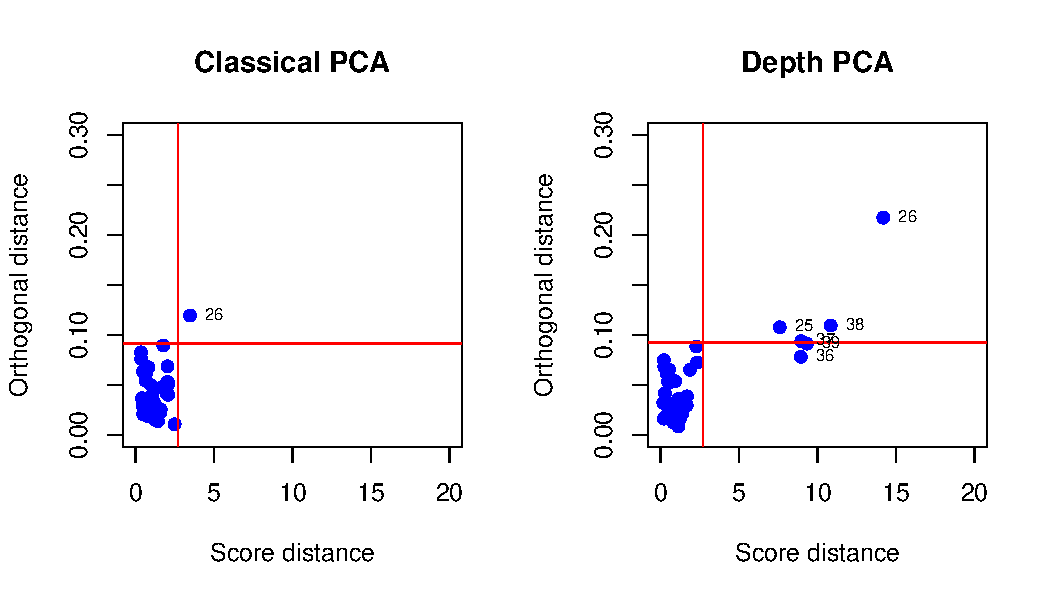
\includegraphics[height=6.5cm]{octane_distanceplot.pdf}
	\caption{Distance plots for two types of PCA on octane data}
	\label{fig:distplot}
\end{figure}